\resizebox{\linewidth}{!}{
\begin{tikzpicture}
    % Colors definition: latexcolor.com
    \definecolor{ashgrey}{rgb}{0.7, 0.75, 0.71}
    \definecolor{x11gray}{rgb}{0.75, 0.75, 0.75}
    \definecolor{metal}{rgb}{0.43, 0.5, 0.5}

    
    % Main outline
    % Background
    \draw[fill=gray!10] (0, 2.75) rectangle (6.75, 6.0);

    % Client Side
    % Client boxes line
    % Client 1
    \draw[fill=gray!5] (0,1.5) rectangle (2, 2.25);
    \node at (1.6, 1.825) {
\includegraphics[width=10pt]{img/smartwatch.png}};
    \node at (1.05, 1.825) {
\includegraphics[width=10pt]{img/wifi-signal.png}};
    \node at (0.4, 1.825) {
\includegraphics[width=15pt]{img/raspberry.png}};
    % Client 2
    \draw[fill=gray!5] (2.5,1.5) rectangle (4.5, 2.25);
    \node at (2.9, 1.825) {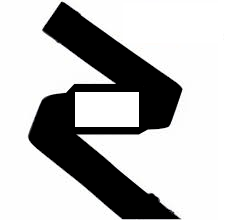
\includegraphics[width=10pt]{img/hrband.png}};
    \node at (3.5, 1.825) {
\includegraphics[width=10pt]{img/wifi-right.png}};
    \node at (4.1, 1.825) {
\includegraphics[width=15pt]{img/raspberry.png}};
    % Client 3
    \node at (5.265, 1.85) {$\cdots$};
    \draw[fill=gray!5] (5.85,1.5) rectangle (6.9, 2.25) node[pos=.5] {\tiny{Client $m$}};
    \draw[fill=gray!5] (8.875,1.5) rectangle (9.625, 2.25) node[pos=.5] {\tiny{Client}};
    % Lines to filesystem
    \draw[<->, dashed, thick] (0.4, 2.25) -- (0.4, 3.5) -- (1, 3.5);
    \draw[<->, dashed, thick] (4.1, 2.25) -- (4.1, 2.35) -- (1.35, 2.35) -- (1.35, 3);
    \draw[<->, dashed, thick] (6.3725, 2.25) -- (6.3725, 2.55) -- (1.85, 2.55) -- (1.85, 3);
    \draw[dashed, thin] (8.875, 2.25) -- (8, 2.75);
    \draw[dashed, thin] (9.625, 2.25) -- (10.5, 2.75);

    % Server Side
    % FileSystem Logo
    \draw[fill=x11gray!50] (1.0, 3) -- (1.1, 3.9) -- (1.6, 3.9) -- (1.75, 4.0) -- (2.1, 4.0) -- (2.0, 3);
    %\draw[fill=x11gray] (1.0, 3) -- (1.0, 3.8) -- (1.6, 3.8) -- (1.75, 3.6) -- (2.0, 3.6) -- (2.0, 3) -- (1.0, 3);
    \node[align=center] at (1.4, 5.1) {\text{\tiny{\textbf{FileSystem}}} \\[-8pt] \text{\tiny{\textbf{Interface}}}};
    % SGX Spark
    % Main Outline
    \draw[fill=white] (2.75, 3) rectangle (6.25, 5.5);
    \node at (4.4, 5.7) {\text{\textbf{\tiny{SGX-Spark Engine}}}};
    % SHM
    \draw (2.95, 3.2) rectangle (6.05, 3.5) node[pos=.5] {\tiny{Host Shared Memory}};
    % Driver
    \draw[pattern=north west lines,pattern color=gray!50] (2.95, 3.7) rectangle (3.95, 4.4); 
    \node at (3.75, 4.5) {\tiny{\texttt{driver-enclave.sh}}};
    \node at (2.95, 3.7) {
\includegraphics[width=8pt]{img/intel-sgx.png}};
    \draw (2.95, 4.6) rectangle (3.95, 5.3); 
    \node at (3.35, 5.4) {\tiny{\texttt{master.sh}}};
    % Worker
    \draw[pattern=north west lines,pattern color=gray!50] (4.15, 3.7) rectangle (6.05, 4.4);
    \node at (4.9, 3.6) {\tiny{\texttt{worker-enclave.sh}}};
    \draw (4.15, 4.6) rectangle (6.05, 5.3);
    \node at (5.55, 5.4) {\tiny{\texttt{worker.sh}}};
    % Tasks Enclave
    \draw[fill=white] (4.25, 3.8) rectangle (4.65, 4.3) node[pos=.5] {\tiny{$T_1$}};
    \draw[fill=white] (4.75, 3.8) rectangle (5.15, 4.3) node[pos=.5] {\tiny{$T_2$}};
    \node at (5.35, 4.05) {\tiny{$\cdots$}};
    \draw[fill=white] (5.55, 3.8) rectangle (5.95, 4.3) node[pos=.5] {\tiny{$T_N$}};
    \node at (6, 3.7) {
\includegraphics[width=8pt]{img/intel-sgx.png}};
    % Tasks Outside Enclave
    \draw (4.25, 4.7) rectangle (4.65, 5.2) node[pos=.5] {\tiny{$T_1$}};
    \draw (4.75, 4.7) rectangle (5.15, 5.2) node[pos=.5] {\tiny{$T_2$}};
    \node at (5.35, 4.95) {\tiny{$\cdots$}};
    \draw (5.55, 4.7) rectangle (5.95, 5.2) node[pos=.5] {\tiny{$T_N$}};

    % CSEM's Toolbox
    \draw[fill=white] (0.8, 3.7) rectangle (2.1, 4.75);
    \node at (1.45, 4.55) {\textsc{\tiny{CSEM HRV}}};
    \draw[dashed] (0.8, 4.4) -- (2.1, 4.4);
    \node[align=left] at (1.42, 4.25) {\texttt{\tiny{+ Identity}}};
    \node[align=left] at (1.19, 4.05) {\texttt{\tiny{+ SDNN}}};
    \node[align=left] at (1.42, 3.85) {\texttt{\tiny{+ HRVBands}}};
    \draw[fill=x11gray] (1.0, 3) -- (1.0, 3.8) -- (1.6, 3.8) -- (1.75, 3.6) -- (2.0, 3.6) -- (2.0, 3) -- (1.0, 3);

    % Client Expansion
    % Separator
    \draw (7.3, 1.5) -- (7.3, 6);
    \draw (7.5, 1.5) -- (7.5, 6);
    % Client itself
    \draw[fill=gray!10] (8, 2.75) rectangle (10.5, 5.55);
    %\draw (9.25, 1.3725) circle (0.5);
    \draw[dashed] (8, 3.55) -- (10.5, 3.55);
    \draw[fill=white] (8.2, 2.95) rectangle (10.3, 3.35) node[pos=.5] {\tiny{\texttt{sensor}}};
    \node at (10.3, 3.00) {
\includegraphics[width=10pt]{img/docker.png}};
    \node at (8.2, 3.00) {
\includegraphics[width=8pt]{img/smartwatch.png}};
    \draw[fill=white] (8.2, 3.75) rectangle (10.3, 4.15) node[pos=.5] {\tiny{\texttt{eclipse-mqtt}}};
    \node at (10.3, 3.80) {
\includegraphics[width=10pt]{img/docker.png}};
    \draw[fill=white] (8.2, 4.35) rectangle (10.3, 4.75) node[pos=.5] {\tiny{\texttt{mqtt-subscriber}}};
    \node at (10.3, 4.40) {
\includegraphics[width=10pt]{img/docker.png}};
    \draw[fill=white] (8.2, 4.95) rectangle (9.2, 5.35) node[pos=.5] {\tiny{\texttt{consumer}}};
    \node at (8.3, 5.00) {
\includegraphics[width=10pt]{img/docker.png}};
    \draw[fill=white] (9.3, 4.95) rectangle (10.3, 5.35) node[pos=.5] {\tiny{\texttt{producer}}};
    \node at (10.3, 5.00) {
\includegraphics[width=10pt]{img/docker.png}};
    \draw[->, very thick, dashed] (9.8, 5.35) -- (9.8, 6);
    \draw[<-, very thick, dashed] (8.7, 5.35) -- (8.7, 6);

\end{tikzpicture}}
